\documentclass[a4paper,ngerman]{tui-algo-seminar}
\usepackage{graphicx}
\usepackage{algorithm2e}
\usepackage{booktabs}
\usepackage{tikz}
\usepackage{hyperref}
\usepackage{float}
\usepackage{amsmath}
\usepackage{listings}
%%\usepackage[margin=1in]{geometry}
\setlength{\footskip}{13.0pt}
\usepackage{thm-restate}

\usepackage[utf8]{inputenc}

\newcommand{\inhalt}{Thüringer Jugend Einzelmeisterschaft 2024}
\seminar{\inhalt}
\semester{\today}
\title{\inhalt}
\author{Erik Skopp}

\usepackage{fancyhdr}
\pagestyle{fancy}
\fancyhf{}
\nolinenumbers

\begin{document}

\maketitle
\thispagestyle{plain}
\begin{abstract}
    Bericht: \inhalt.\\
    Vom 4. bis zum 7. April fand in Naumburg (Sachsen-Anhalt) die diesjährige Thüringer Jugend-Einzelmeisterschaft im Schach statt. In jeder Altersklasse wurden sieben Runden nach dem Schweizer System ausgetragen. Die Gewinner qualifizieren sich für die Deutsche Einzelmeisterschaft in Willingen.
\end{abstract}

%\listoffigures
%\listoftables
\tableofcontents 

\clearpage

\section{Bericht}


\subsection{Einleitung}

\subsection{Turnier}

\subsection{Hanna Görlach}
Hanna Görlach, die das Turnier mit einer Turnierwertungszahl von 1122 antrat, hatte sichtlich mit den hohen Erwartungen zu kämpfen. Ihre Partien offenbarten Momente brillanter Strategie und den Anflug dessen, was möglich gewesen wäre. Doch trotz erkennbarer Entschlossenheit und intensiver Konzentration blieben die Ergebnisse hinter den Möglichkeiten zurück. Mit jeder Runde, in der ein potenzieller Sieg durch ihre Finger zu gleiten schien, wuchs das Gefühl, dass dieses Turnier mehr eine Reihe verpasster Chancen war. Görlachs Bemühungen waren nicht von Erfolg gekrönt, und es lässt sich nur erahnen, wie sehr sie diese Momente nach dem Ende einer jeden Partie reflektiert haben muss. Es bleibt die Hoffnung, dass sie diese Erfahrungen als wertvolle Lektionen für zukünftige Turniere nutzen und die verdiente Wende herbeiführen kann.


\subsection{Ronika, Nasiri}
In der U10 weiblich vertrat uns Kashvi Ray. Mit einer TWZ von 758 hatte sie die dritt geringste Wertungszahl in ihrer Altersklasse. Die U10 bestand aus 12 Teilnehmern.  In der ersten Runde konnte Sie mit einem Weißsieg über Cäcilia Ulbrich einen wichtigen Sieg erringen. In Runde zwei und drei hatte Ronika leider nicht so viel Glück und musste sich Amalia und Amelia geschlagen geben. Beide hatten eine höhere Wertungszahl als Ronika. In Runde vier wendete sich das Blatt und es gelang ihr ein Sieg gegen Elenor von Blau Weiß Stadtilm. In Runde fünf verlor sie unglücklich gegen Julia aus Saalfeld. Am letzten Spieltag sammelte Ronika noch einmal ihre Kraft und erkämpfte sich sowohl in Runde sechs und sieben ein Remis gegen Fenja Nöthlich und Emiliy Fischer. Damit erreichte sie 3 Punkte aus 7 Spielen und einen stark durchwachsenen neunten Platz. Ihre DWZ konnte sie dabei leider nicht bestätigen und verlor 20 Punkte und rutsch damit von einer 758 auf eine 738 ab. Leider war mit dieser Leistung eine Qualifikation für die Deutsche Meisterschaft nicht möglich, jedoch konnte sie viel Lernen und im kommenden jahr angreifen und die Altersklasse dominieren.


\subsection{Kashvi Ray}


\subsection{Zusammenfassung}


\subsection{Abschluss}


\clearpage
\section{Tabellen}
Alle Tabellen entstammen der Veröffentlichung der Thüringer Schachjugend unter folgender URL \url{https://ed.thsj.de/index.php/them-2024}\footnote{Der LInk wurde am \today ~abgerufen.}

% Auch wenn die Pfade nicht stimmen findet Overleaf die Projekte. Bei GitHub und dem Worfkflow ist das nicht so,
\subsection{Hanna Görlach}
    \subsubsection{Partien}
        \begin{table}[htbp]
\centering
\caption{Turnier Rangliste}
\begin{tabular}{|l|c|l|l|c|c|}
\hline
\multicolumn{6}{|c|}{Partien} \\
\hline
Runde & Farbe & Spieler & Verein & ELO & Ergebnis \\
\hline
1 & W & Grube, Anna (2.5) & ESV Lok Meiningen & 841 & 1 \\
2 & S & Brauer, Celiene (4) & SC Turm Erfurt & 1172 & 0.5 \\
3 & S & Ignatova, Gabriela (4.5) & Meuselwitzer SV & 1464 & 0.5 \\
4 & W & Richter, Amélie Elsa (4) & SG Blau-Weiß Stadtilm & 1205 & 0 \\
5 & W & Huth, Fabienne (4) & VfL 1990 Gera & 1072 & 0.5 \\
6 & S & Zeughardt, Selma (3) & Erfurter SK & 1006 & 0.5 \\
7 & W & Scheiding, Sophia (4.5) & Meuselwitzer SV & 1470 & 0 \\
\hline
\multicolumn{4}{|r|}{Gesamt} & Ø 1175 & 3.0 / 5, 13. Platz \\
\hline
\end{tabular}
\end{table}

\section{Bilder}
Bitte keine Bilder von Hanna auf die Website des Ilmenauer SV's\footnote{\url{https:ilmenauer-schachverein.de}} hochladen.
\vspace{0.5cm}
Alle Bilder finden Sie in der Cloud. Bitte nutzen Sie diese. Wir haben von Norbert Reichel via E-Mail die Rechte die Bilder für die Berichte zu nutzen. \\
Die Berechtigung liegt ab dem 19.04 dem Vorstand des Ilmenauer Schachvereines (Markus Hartung) vor.f
    \subsubsection{Rangliste U14w-U18w}
        \begin{table}[H]
\centering
\begin{tabular}{|c|l|l|l|c|c|c|c|c|c|}
\hline
Nr. & Titel & Spieler & Verein & TWZ & Sp & Pkt & BhZl-1 & SoBe-1 & + \\ \hline
1 & 16w & Eichhorn, Mathilda & SV Schott Jena & 1737 & 7 & 5.5 & 27.5 & 21.25 & 4 \\
2 & 18w & Ulrich, Helena Irene & SV Medizin Erfurt & 1732 & 7 & 5.5 & 27.0 & 19.75 & 4 \\
3 & 16w & Loos, Tilda & VfL 1990 Gera & 1500 & 7 & 5.0 & 26.5 & 17.25 & 3 \\
4 & 14w & Ignatova, Gabriela & Meuselwitzer SV & 1464 & 7 & 4.5 & 26.0 & 15.25 & 2 \\
5 & 16w & Scheiding, Sophia & Meuselwitzer SV & 1470 & 7 & 4.5 & 24.0 & 14.75 & 4 \\
6 & 16w & Niederdorfer, Mathilda & SV Empor Erfurt & 1257 & 7 & 4.0 & 27.0 & 14.00 & 3 \\
7 & 16w & Richter, Amélie Elsa & SG Blau-Weiß Stadtilm & 1205 & 7 & 4.0 & 24.5 & 12.00 & 4 \\
8 & 16w & Huth, Fabienne & VfL 1990 Gera & 1072 & 7 & 4.0 & 20.5 & 9.50 & 3 \\
9 & 16w & Brauer, Celiene & SC Turm Erfurt & 1172 & 7 & 4.0 & 20.0 & 10.75 & 3 \\
10 & 16w & Wicklein, Isabella & fuß brothers Jena & 941 & 7 & 3.5 & 20.5 & 10.25 & 3 \\
11 & 14w & Fota, Heidi & SV Empor Erfurt & 917 & 7 & 3.5 & 20.0 & 7.50 & 3 \\
12 & 14w & Le, Thi An & 1. Eichsfelder SC & 1105 & 7 & 3.5 & 19.5 & 7.00 & 3 \\
13 & 18w & Görlach, Hanna & Ilmenauer SV & 1122 & 7 & 3.0 & 24.0 & 10.25 & 1 \\
14 & 14w & Zeughardt, Selma & Erfurter SK & 1006 & 7 & 3.0 & 22.5 & 9.50 & 2 \\
15 & 14w & Stadelmann, Henriette & SSV Vimaria 91 Weimar & 1041 & 7 & 3.0 & 22.0 & 7.75 & 2 \\
16 & 14w & Grube, Anna & ESV Lok Meiningen & 841 & 7 & 2.5 & 24.0 & 5.75 & 2 \\
17 & 14w & Dilcher, Maria & SV Empor Erfurt & 804 & 7 & 2.5 & 23.5 & 5.00 & 2 \\
18 & 16w & Yusibova, Shams & SV Empor Erfurt & 999 & 7 & 2.5 & 20.5 & 5.00 & 2 \\
19 & 14w & Yusibova, Banu & SV Empor Erfurt & 976 & 7 & 2.0 & 20.5 & 3.00 & 1 \\ \hline
\end{tabular}
\caption{Rangliste U14w-U18w}
\label{tab:Rangliste_U14w-U18w}
\end{table}
\clearpage

\subsection{Kashvi Ray}
    \subsubsection{Partien}
        \begin{table}
\begin{tabular}{|c|c|l|l|c|}
\hline
\textbf{Partien} & \textbf{Runde} & \textbf{Spieler} & \textbf{Verein} & \textbf{Punkte} \\ \hline
S & Runde 1 & Ulbrich, Cäcilia (4) & 1. Eichsfelder SC & 1 \\ \hline
S & Runde 2 & Sniegowski, Amalia (6) & Meuselwitzer SV & 0 \\ \hline
W & Runde 3 & Buntin, Amelia Bernadette (5) & ZSG Grün-Weiß Waltershausen & 0 \\ \hline
S & Runde 4 & Nawatzki, Elenor Viktoria (1) & SG Blau-Weiß Stadtilm & 1 \\ \hline
S & Runde 5 & Heß, Julia (3.5) & MTV 1876 Saalfeld & 0 \\ \hline
W & Runde 6 & Nöthlich, Fenja (0.5) & SV Empor Erfurt & 0.5 \\ \hline
S & Runde 7 & Fischer, Emily (2.5) & SV Springer Oldisleben & 0.5 \\ \hline
\multicolumn{4}{|r|}{\textbf{Gesamt (3 Spieler)}} & \textbf{3.0/4} \\ \hline
\multicolumn{4}{|r|}{\textbf{Durchschnitt}} & \textbf{861} \\ \hline
\multicolumn{4}{|r|}{\textbf{Platz}} & \textbf{9.} \\ \hline
\end{tabular}
\caption{Partien Kashvi}
\label{label:Tabelle_Kashvi}
\end{table}
    \subsubsection{Rangliste U10w}
        \begin{table}[H]
\centering
\begin{tabular}{|c|l|l|c|c|c|c|c|c|}
\hline
Nr. & Spieler & Verein & TWZ & Sp & Pkt & BhZl-1 & SoBe-1 & + \\ \hline
1 & Sniegowski, Amalia & Meuselwitzer SV & 975 & 7 & 6.0 & 24.5 & 22.50 & 6 \\
2 & Buntin, Amelia Bernadette & ZSG Grün-Weiß Waltershausen & 887 & 7 & 5.0 & 26.0 & 18.50 & 5 \\
3 & Fritzsche, Emma & SV Empor Erfurt & - & 7 & 4.5 & 26.5 & 15.75 & 3 \\
4 & Eßers, Mathilda Marie & SG Blau-Weiß Stadtilm & 924 & 7 & 4.5 & 24.0 & 13.25 & 4 \\
5 & Möller, Lia Sofie & SG Blau-Weiß Stadtilm & 733 & 7 & 4.0 & 26.0 & 14.50 & 4 \\
6 & Ulbrich, Cäcilia & 1. Eichsfelder SC & - & 7 & 4.0 & 19.0 & 7.50 & 4 \\
7 & Beier, Viktoria & SV Empor Erfurt & - & 7 & 3.5 & 24.5 & 7.75 & 3 \\
8 & Heß, Julia & MTV 1876 Saalfeld & 723 & 7 & 3.5 & 23.5 & 8.25 & 3 \\
9 & Ray, Kashvi & Ilmenauer SV & 758 & 7 & 3.0 & 22.0 & 6.50 & 2 \\
10 & Fischer, Emily & SV Springer Oldisleben & - & 7 & 2.5 & 21.5 & 3.00 & 2 \\
11 & Nawatzki, Elenor Viktoria & SG Blau-Weiß Stadtilm & - & 7 & 1.0 & 22.0 & 0.50 & 1 \\
12 & Nöthlich, Fenja & SV Empor Erfurt & - & 7 & 0.5 & 21.0 & 1.50 & 0 \\ \hline
\end{tabular}
\caption{Rangliste U10w}
\label{tab:Rangliste_U10w}
\end{table}
\clearpage

\subsection{Ronika Nasiri}
    \subsubsection{Partien}
        \begin{table}[htbp]
\centering
\caption{Turnier Rangliste U12}
\begin{tabular}{|l|c|p{1.8in}|l|c|c|}
\hline
\multicolumn{6}{|c|}{Partien} \\
\hline
\textbf{Runde} & \textbf{Farbe} & \textbf{Spieler} & \textbf{Verein} & \textbf{ELO} & \textbf{Ergebnis} \\
\hline
1 & S & Ulbrich, Eusebia (4.5) & 1. Eichsfelder SC & 810 & 0 \\
2 & S & Weichel, Juliette (3.5) & SV Empor Erfurt & 778 & 0 \\
3 & W & Kührt, Daria (3.5) & SV Empor Erfurt & --- & 1 \\
4 & W & Böttcher, Paulina (2) & SV Springer Oldisleben & 788 & 0 \\
5 & S & Lehmann, Clara Theres (3) & SV Empor Erfurt & 935 & 0 \\
6 & W & Liebaug, Ellen (1.5) & SC Rochade Steinbach-Hallenberg & --- & 1 \\
7 & S & Hoyer, Clara (4) & SV Empor Erfurt & 798 & 0 \\
\hline
\multicolumn{4}{|r|}{Gesamt} & Ø 821 (5 Spieler) & 2.0 / 2, 12. Platz \\
\hline
\end{tabular}
\end{table}
    \subsubsection{Rangliste U12w}
        \begin{table}[H]
\centering
\begin{tabular}{|c|l|l|c|c|c|c|c|c|}
\hline
Nr. & Spieler & Verein & TWZ & Sp & Pkt & BhZl-1 & SoBe-1 & + \\ \hline
1 & Schille, Marlene & VfL 1990 Gera & 1125 & 7 & 6.0 & 25.5 & 20.50 & 5 \\
2 & Albrecht, Sidney Jenna & SV Empor Erfurt & 1295 & 7 & 5.5 & 26.5 & 21.50 & 5 \\
3 & Sniegowski, Victoria & Meuselwitzer SV & 1019 & 7 & 5.0 & 24.5 & 18.50 & 5 \\
4 & Ulbrich, Eusebia & 1. Eichsfelder SC & 810 & 7 & 4.5 & 27.5 & 16.00 & 4 \\
5 & Weißleder, Emia & SV Empor Erfurt & 1086 & 7 & 4.0 & 24.5 & 10.00 & 4 \\
6 & Hoyer, Clara & SV Empor Erfurt & 798 & 7 & 4.0 & 22.5 & 10.25 & 3 \\
7 & Weichel, Juliette & SV Empor Erfurt & 778 & 7 & 3.5 & 23.5 & 9.00 & 3 \\
8 & Kührt, Daria & SV Empor Erfurt & - & 7 & 3.5 & 17.0 & 6.50 & 3 \\
9 & Lehmann, Clara Theres & SV Empor Erfurt & 935 & 7 & 3.0 & 22.5 & 5.00 & 3 \\
10 & Gallerach, Elisa & ESV Lok Sömmerda & 916 & 7 & 3.0 & 21.5 & 6.75 & 2 \\
11 & Böttcher, Paulina & SV Springer Oldisleben & 788 & 7 & 2.0 & 22.0 & 5.00 & 2 \\
12 & Nasiri, Ronika & Ilmenauer SV & - & 7 & 2.0 & 20.5 & 5.00 & 2 \\
13 & Burkhardt, Charlotte & SC Rochade Steinbach-Hallenberg & - & 7 & 1.5 & 22.5 & 5.75 & 1 \\
14 & Liebaug, Ellen & SC Rochade Steinbach-Hallenberg & - & 7 & 1.5 & 18.5 & 2.75 & 1 \\ \hline
\end{tabular}
\caption{Turniertabelle}
\label{tab:turniertabelle}
\end{table}

    
\clearpage


\section{Bilder}
Die Fotografien von Markus Hartung und Norbert Reichel für die Veranstaltung sind unter folgender Cloud-Adresse verfügbar: \url{https://cloud.ilmenauer-schachverein.de/apps/files/files/72384?dir=/Events/2024_04_THJEM/Bilder}. Wir haben die Erlaubnis erhalten, diese Bilder im Rahmen unserer Öffentlichkeitsarbeit zu nutzen. Die Genehmigung von Norbert Reichel wurde eingeholt und kann per E-Mail unter \href{mailto:info@ilmenauer-schachverein.de}{info@ilmenauer-schachverein.de} bestätigt werden.

Bitte beachten Sie die Bitte von Hanna Görlach, keine Bilder von ihr auf der Webseite des Ilmenauer Schachvereins oder auf Instagram zu veröffentlichen, entsprechend ihrem ausdrücklichen Wunsch. 

\subsection{Bild 1 - Kashvi am Brett}
\begin{center}
    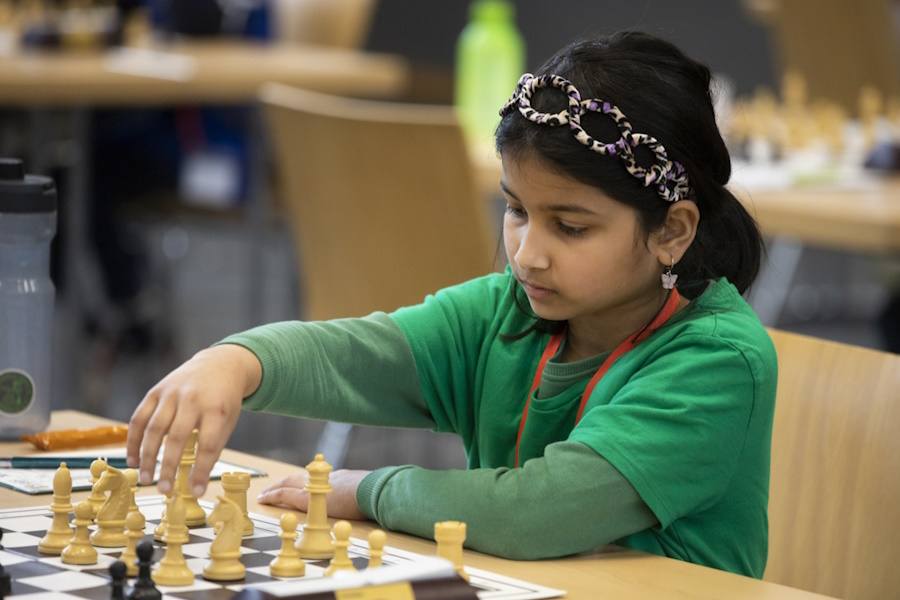
\includegraphics[width=\linewidth,height=0.5625\linewidth,keepaspectratio]{THJEM2.jpg}
    \captionof{figure}{Kashvi Bild}
    \label{fig:Kashvi Bild}
\end{center}

\subsection{Bild 2 - Hanna gegen Anna in Runde 1}
\begin{center}
    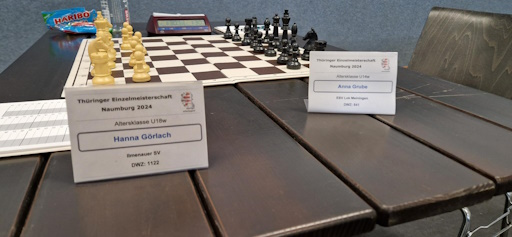
\includegraphics[width=0.8\linewidth,height=0.45\linewidth,keepaspectratio]{THJEM1.jpeg}
    \captionof{figure}{THJEM Hanna Schild}
    \label{fig:THJEM Hanna Schild}
\end{center}



\end{document}
